\chapter{Implementation}
\label{ch:implementation}
\begingroup
\sloppy
\setlength{\emergencystretch}{3em}

This chapter presents how the framework design from Chapter~3 is realized in source code: the implementation environment and configuration, the framework module organization, the shared runtime and utility layer, the UI and API automation implementations, the reporting and debugging configuration, and the Copilot-supported automation-testing workflow. Throughout, it reports evidence at the level of source structure and configuration; verified execution results and their interpretation are reserved for Chapter~5.

\section{Implementation Environment and Configuration}
\label{sec:ch4-implementation-environment-configuration}

The implementation is organized as a Playwright and TypeScript automation framework. The package manifest defines \code{@playwright/test}, \code{playwright}, TypeScript-related Node typings, \code{dotenv}, and \code{ajv} as the main dependencies used for browser automation, API request support, environment-variable loading, and JSON-schema validation utilities. The project documentation describes direct command-line execution through \code{npm install}, \code{npx playwright test}, \code{npx playwright test --headed}, \code{npx playwright test --debug}, and \code{npx playwright show-report}. Because the current package manifest does not define npm script aliases, the implementation is described through these direct Playwright commands rather than through project-specific script names.

The central configuration is implemented in \path{playwright.config.ts}. It loads environment variables from \path{config/.env}, uses \code{process.env.BASE_URL} as the browser base URL, and works with \path{utils/api-url.ts}, which constructs API URLs from \code{process.env.API_BASE_URL}. This study records these mechanisms at the configuration and variable-name level only. It does not disclose runtime values, access tokens, client identifiers, or credential data.

The Playwright configuration sets \code{testDir: './tests'}, so both UI and API specifications are discovered under the shared test directory. It defines a Chromium project with Playwright's desktop Chrome device settings, a global timeout of \code{10 * 60 * 1000}, an action timeout of \code{10 * 1000}, full parallel execution, CI-only \code{forbidOnly}, two retries in CI, and a single worker in CI \autocite{playwright_docs_configuration_2026}. These values document the runtime configuration rather than any measured reliability or performance outcome.

\section{Implemented Framework Organization}
\label{sec:ch4-implemented-framework-organization}

The implemented framework follows the layered design introduced in Chapter~3, described here at the level of concrete source organization. UI and API test specifications are implemented under \path{tests/ui/} and \path{tests/api/}. UI interaction logic is implemented in Page Object classes under \path{page-object/}, reusable business flows are implemented under \path{workflow/}, and fixture definitions are implemented under \path{fixtures/} and \path{core/fixtures/}.

API-related implementation is separated into service classes under \path{api-service/}, endpoint constants under \path{constants/}, request and response models under \path{data-object/}, and reusable request utilities under \path{core/api/}. Browser runtime utilities and element wrappers are implemented under \path{core/browser/} and \path{core/element/}, while shared helpers for JSON loading and API URL construction are placed under \path{utils/}. This organization allows test specifications to focus on scenario behavior while reusable framework components handle interaction, request construction, runtime access, and data management.

\Cref{fig:vscode-test-explorer-playwright-panel} provides a development-environment view of the implemented test organization. The VS Code Test Explorer shows the API and UI test specifications grouped under the shared \path{tests} directory, while the Playwright panel exposes tooling actions such as locator picking, recording, report output access, and trace-viewer settings. The figure is included as implementation-context evidence only; it does not replace the verified execution results presented in Chapter~5.

\begin{figure}[htbp]
  \centering
  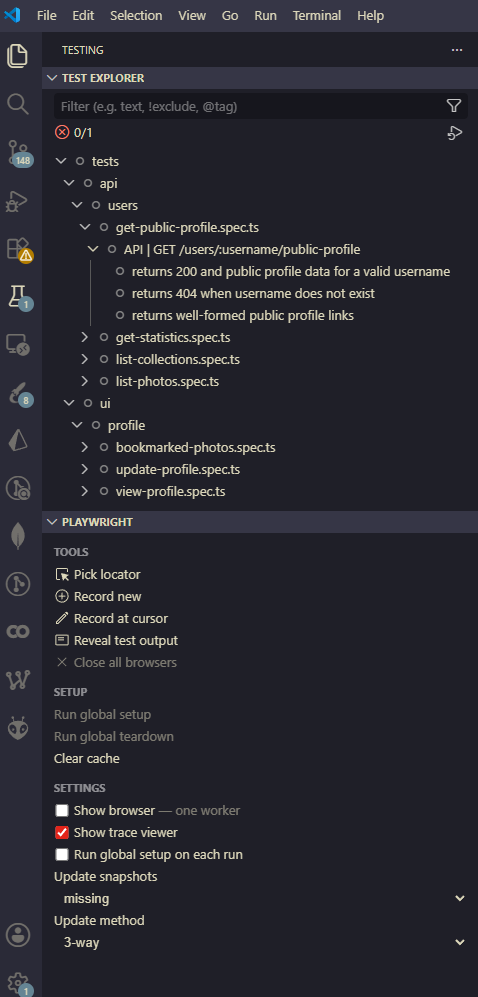
\includegraphics[width=0.92\textwidth,height=0.75\textheight,keepaspectratio]{figures/screenshots/vscode-test-explorer-playwright-panel.png}
  \caption{VS Code Test Explorer and Playwright panel showing the implemented API and UI test organization.}
  \label{fig:vscode-test-explorer-playwright-panel}
\end{figure}

\section{Runtime and Utility Implementation}
\label{sec:ch4-runtime-utility-implementation}

The runtime utility layer provides the shared operational support used by both UI and API tests. \path{core/browser/browser-management.ts} stores references to the active Playwright browser, browser context, page, and API request context after fixture initialization. This allows browser utilities, element wrappers, and API utilities to access the active runtime objects through a single framework utility layer.

The fixture implementation makes these runtime objects and reusable abstractions available to tests. The custom fixture extends the base fixture and injects \code{HomePage}, \code{LoginPage}, \code{ProfilePage}, \code{AccountPage}, \code{LoginWorkflow}, \code{LikePage}, \code{CollectionPage}, and \code{BookmarkPage} into test functions \autocite{playwright_docs_fixtures_2026}. This implementation realizes the runtime composition design discussed in Chapter~3 at the source-code level.

Two utility implementations are especially relevant to the representative scenarios. First, \path{core/element/element.ts} wraps Playwright locator access and common element operations, including clicks, fills, visibility waits, text retrieval, attribute access, and visibility assertions \autocite{playwright_docs_locators_2026}. Second, \path{core/api/api.ts} implements reusable \code{get()}, \code{post()}, \code{put()}, and \code{delete()} methods through the active Playwright request context \autocite{playwright_docs_apirequestcontext_2026}. The same API utility also contains helper methods for security-header checks and JSON-schema validation through Ajv. These helpers exist in the framework, but their presence alone does not constitute broad security or schema-validation coverage; such a claim would require dedicated test evidence.

\section{UI Automation Implementation}
\label{sec:ch4-ui-automation-implementation}

The UI automation implementation is represented most clearly by the profile-related specifications under \path{tests/ui/profile/}. These tests use fixture-injected Page Objects and workflows rather than constructing page abstractions directly inside each specification. The implemented Page Object layer includes representative classes such as \code{HomePage}, \code{LoginPage}, \code{ProfilePage}, and \code{AccountPage}, with additional page abstractions such as \code{LikePage}, \code{CollectionPage}, and \code{BookmarkPage} made available through fixtures for related profile and photo interactions.

The login workflow is implemented in \path{workflow/login-workflow.ts}. It composes \code{LoginPage}, \code{HomePage}, and \code{BrowserUtils} to navigate to the login page, submit credentials through the login page abstraction, and wait for the home page avatar image to become visible. This implementation turns a repeated authenticated setup sequence into a reusable workflow that can be consumed by tests through fixture injection.

The update-profile scenario provides the most complete UI implementation example. The test loads user data through \code{JsonHelper.getUserInfo('valid_account')}, logs in through \code{loginWorkflow.login()}, navigates to the user profile through \code{HomePage}, opens the edit-profile page through \code{ProfilePage}, changes the username through \code{AccountPage}, submits the form, and checks that the update success message is visible. After the UI state change, the test navigates to the updated profile URL through \code{BrowserUtils.navigate()} and verifies the visible profile full name against the account first and last name. This demonstrates how the implementation combines fixture injection, Page Objects, workflow reuse, shared test data, browser navigation, and UI assertions in one representative scenario.

The same test defines an \code{afterEach} cleanup hook. It creates an \code{UpdateUserProfileRequestData} object, restores the original username, and calls \code{UsersService.updateCurrentUserProfile()} with the access token loaded from centralized user data. This is implementation evidence of API-assisted cleanup after a state-changing UI scenario. Its long-term reliability is assessed in Chapter~5 rather than inferred from the source code alone.

\section{API Automation Implementation}
\label{sec:ch4-api-automation-implementation}

The API automation implementation is represented by user endpoint tests under \path{tests/api/users/} and service classes under \path{api-service/}. \code{UsersService} centralizes public user profile retrieval, user photos, user collections, user statistics, and current-user profile update operations. Endpoint paths are imported from \path{constants/api-endpoints.ts}, and full URLs are constructed through \path{utils/api-url.ts}. \code{PhotosService} follows the same service-oriented style for retrieving random photos and performing like or unlike operations.

The service implementation also centralizes public-read authorization behavior. When an access token is provided, \code{UsersService} uses bearer-token authorization. When an access token is not supplied, it attempts to use an Unsplash access key or client identifier from environment variables. This study describes the mechanism only as an implementation pattern and does not disclose token or key values.

The representative API specification is \path{tests/api/users/get-public-profile.spec.ts}. It imports \code{UsersService}, reads an access token from centralized user data, and calls \code{UsersService.getUserPublicProfile()}. The test validates a successful public profile response, an invalid-username \code{404} response, and expected URL patterns in profile links. It also contains source-level handling for public API rate-limit text. This supports describing how the API suite is implemented around service methods and response assertions, while actual pass/fail results remain part of the Chapter~5 evaluation evidence.

\section{Reporting and Debugging Configuration}
\label{sec:ch4-reporting-debugging-configuration}

Reporting and debugging support is implemented through Playwright configuration and documented execution commands. The configuration enables the Playwright HTML reporter, a JUnit reporter with \code{results.xml} as the configured output file, and trace collection on first retry \autocite{playwright_docs_reporters_2026,playwright_docs_trace_viewer_2026}. The README documents \code{npx playwright show-report} for viewing the generated HTML report after execution.

\Cref{fig:playwright-reporting-pipeline} summarizes the reporting pipeline as an implementation-level configuration mechanism.

\begin{figure}[htbp]
  \centering
  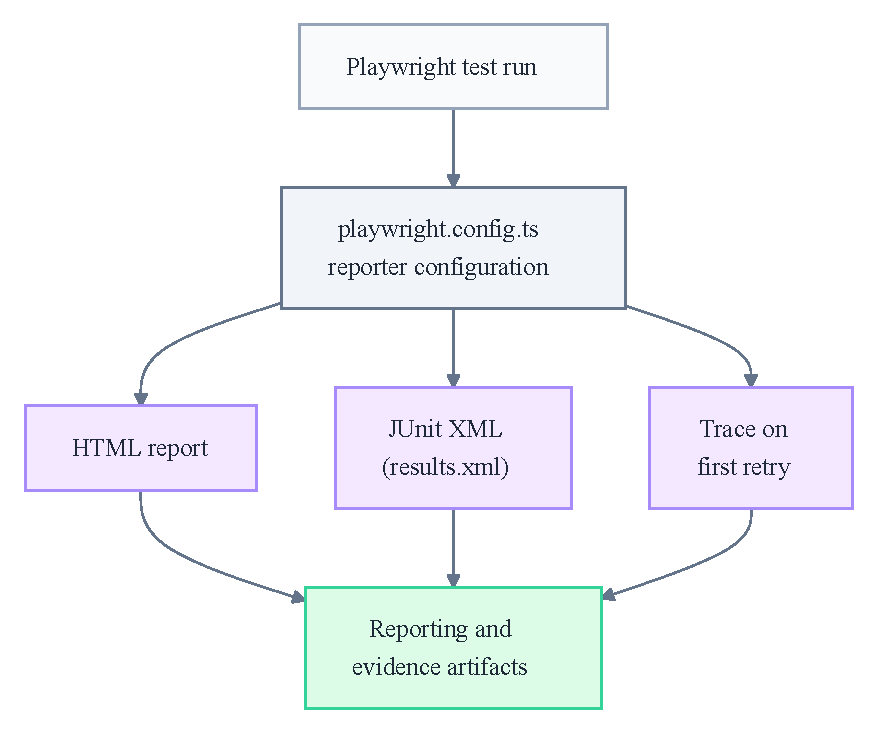
\includegraphics[width=\textwidth,height=0.8\textheight,keepaspectratio]{figures/workflows/playwright-reporting-pipeline.pdf}
  \caption{Playwright execution and reporting pipeline.}
  \label{fig:playwright-reporting-pipeline}
\end{figure}

Verified execution evidence from the 2026-06-03 local full-suite run is presented in Chapter~5, including the HTML report screenshot and JUnit XML evidence. Because the full-suite run passed without retry, it did not produce a trace under the configured \code{trace: 'on-first-retry'} setting. A supplemental trace zip exists for one representative UI run; the supplemental trace artifact has been loaded, sanitized, and is presented as \cref{fig:playwright-trace-viewer} in Chapter~5 and referenced in \hyperref[app:sample-reports]{Appendix~D}.

\section{Copilot-Supported Automation Workflow Implementation}
\label{sec:ch4-copilot-supported-automation-workflow-implementation}

The project also implements a documentation-driven Copilot Agentic-AI workflow that supports automation testing development. This workflow is represented by project artifacts under \path{docs/agentic-workflow/}, \path{.github/}, and \path{.claude/}; it supports repository understanding, automation-ready scenario design, framework-aware Playwright script generation, and generated-code review. This section treats the workflow as a support layer around the Playwright framework, not as evidence of measured productivity improvement or defect reduction.

The repository-wide instruction layer is implemented through \path{.github/copilot-instructions.md}, which records framework conventions such as the reuse-first policy, Page Object expectations, fixture usage, workflow placement, API service rules, test file placement, naming guidance, and Playwright MCP preference when UI understanding or selector validation is uncertain. The agent and prompt layers are implemented through \path{.github/AGENTS.md}, \path{.github/agents/}, and \path{.github/prompts/}, including scenario-design, script-generation, and generated-code review entry points.

\Cref{fig:copilot-script-generation-workflow} shows the implemented workflow for framework-aware script generation.

\begin{figure}[htbp]
  \centering
  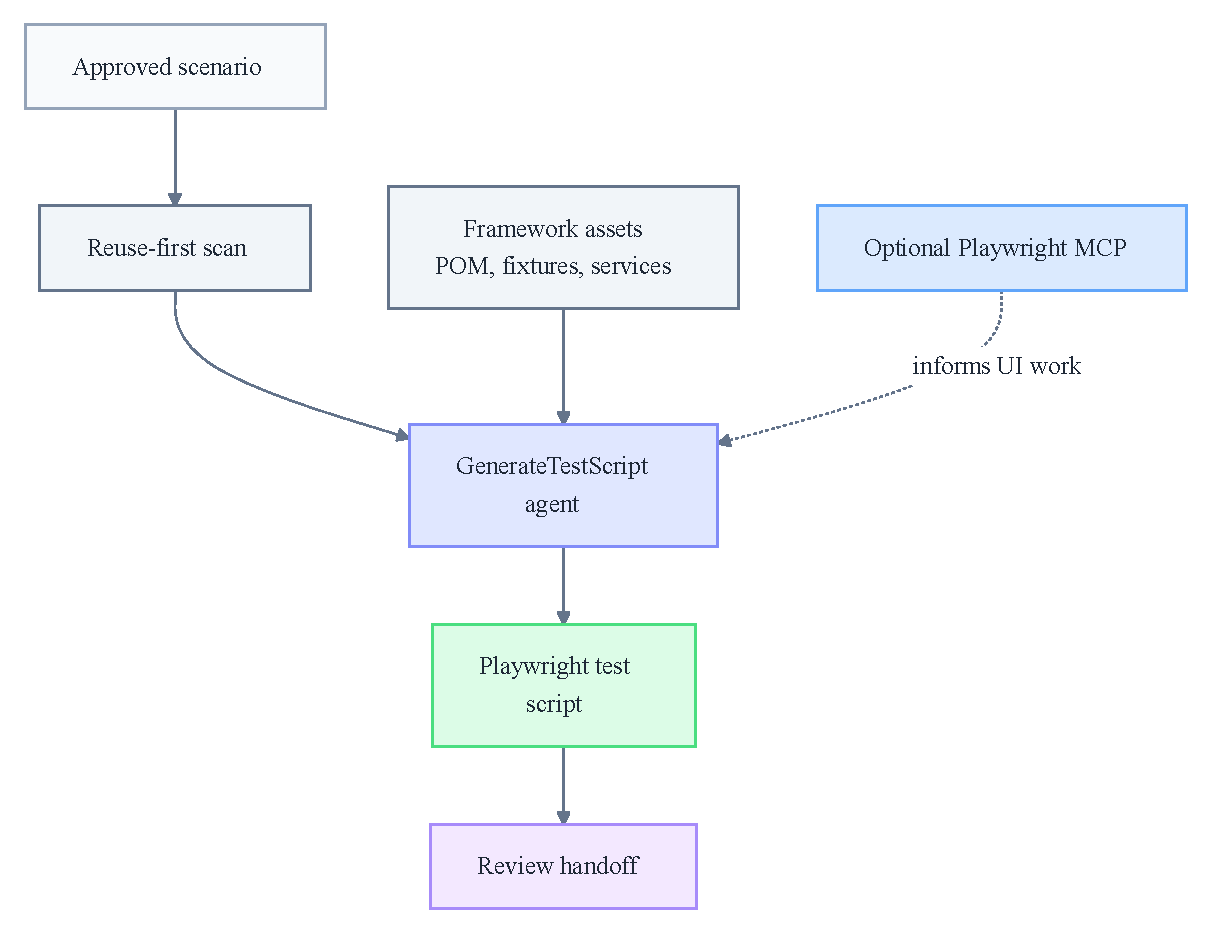
\includegraphics[width=\textwidth,height=0.8\textheight,keepaspectratio]{figures/workflows/copilot-script-generation-workflow.pdf}
  \caption{Copilot-supported Playwright script-generation workflow.}
  \label{fig:copilot-script-generation-workflow}
\end{figure}

The reusable skill layer is stored under \path{.claude/skills/}. The \code{playwright-mcp} skill supports browser and DOM inspection, the \code{script-generation} skill supports framework-aware generation guidance, the \code{design-test-case} skill supports automation scenario design, and the \code{code-review} folder contains review references for maintainability, Page Object quality, and selector quality. \Cref{fig:copilot-code-review-workflow} summarizes the generated-code review workflow.

\begin{figure}[htbp]
  \centering
  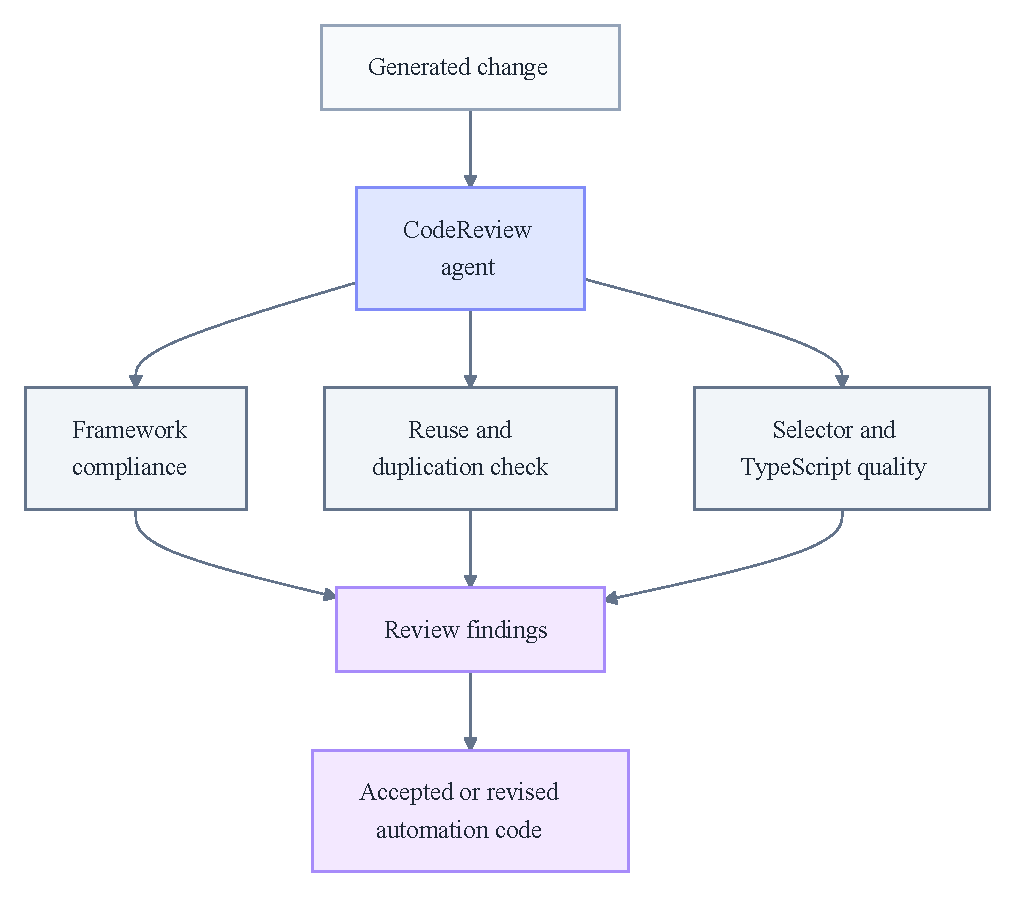
\includegraphics[width=\textwidth,height=0.8\textheight,keepaspectratio]{figures/workflows/copilot-code-review-workflow.pdf}
  \caption{Copilot-supported automation code-review workflow.}
  \label{fig:copilot-code-review-workflow}
\end{figure}

The implementation evidence is strongest for the generated-code review workflow in \path{.github/AGENTS.md}, \path{.github/prompts/review-generated-script.prompt.md}, and the reference materials under \path{.claude/skills/code-review/references/}. The source note records a documentation consistency risk in \path{.claude/skills/code-review/SKILL.md}, whose main content appears less aligned with the folder name than its reference files. For this reason, the thesis describes the workflow as a documented support mechanism and avoids claims about quantitative effectiveness, quality improvement, or execution reliability without a separate evaluation method.
\endgroup
